%!TEX root = ../main/main.tex
\subsection{Análise do Componente Principal}
\subsubsection{Padronização das variáveis}

De acordo com \citeonline[p.~98]{larose2015data} a padronização dos dados precede a aplicação da Análise do Componente Principal - ACP (ou \textit{Principal Component Analysis}). Isso fica evidente com base na observação da sumarização estatística apresentada na tabela \ref{tbl: sumario-estatisico-com-knn}. Nesta tabela é possível observar a desproporcionalidade dos desvios-padrão entre as variáveis. Concluintes Inscritos, por exemplo, tem um desvio 896 vezes maior que Nota Bruta - Regime de Trabalho. Ainda de acordo com o mesmo autor, a padronização tem como principal objetivo evitar que a influência de uma variável domine a da outra no espectro de variabilidade.

Tanto a ACP como a AF (Análise do Fator, como será visto adiante) fizeram amplo uso do pacote \lstinline{psych}\footnote{Possui ferramentas estatísticas de propósito geral para aplicações em psicometria, personalidade e psicologia experimental.}. Dada a sua importância, este pacote constitui elemento chave para a aplicação das metodologias estatísticas desta pesquisa. De acordo com \citeonline{psych}, abarca um conjunto de funções para análise multivariada permitindo a criação de estatísticas descritivas. Dentre estas funções podem ser destacadas \lstinline{fa} e \lstinline{principal} que possibilitaram a computação dos carregamentos para a AF e ACP, respectivamente.

A padronização dos dados foi feita com a utilização da função \lstinline{scales} contida na instalação básica do R. Esta função posiciona as variáveis contínuas em uma unidade de escala pela subtração de sua média e divisão pelo desvio padrão (procedimento denominado \textit{z-scoring}). Isso torna o desvio padrão das mesmas 1 e a média 0. Em termos matemáticos a padronização pode ser expressa pela seguinte equação: 

\begin{equation}
Z_{i}=\dfrac{X_{i}-\mu_{i}}{\sigma_{ii}}
\end{equation}

Foi observado que o \textit{dataset} do CPC contém, para cada nota bruta, uma nota padronizada. Além disso, segundo \citeonline{INEP_2017} a metodologia utilizada para produção destas notas é expressa pela seguinte equação: 

\begin{equation}
Z_{FGj}=\dfrac{FG_{kj}-\overline{FG}_k}{S_{FGk}}
\end{equation}


Onde,

\begin{itemize}[label={}]
\item $Z_{FGj}$ é o afastamento padronizado em $FG$ da unidade de observação $j$;
\item $FG_{kj}$ é a nota bruta em $FG$ da $j$-ésima unidade de observação da área de avaliação $k$;
\item $\overline{FG}_k$ é a média em $FG$ da área de avaliação $k$; e
\item $S_{FGk}$ é o desvio-padrão em $FG$ da área de avaliação $k$.
\end{itemize}

Nesta pesquisa optou-se por manter tais variáveis no conjunto de preditoras. Esta decisão foi tomada com base na verificação de que tal metodologia é aplicada para a composição da respectiva variável. Além do mais, a mesma não necessariamente implica em desvio padrão unitário e média 0 quando a análise é feita sobre a totalidade de observações, como pode ser observado na tabela \ref{tbl: vars-padronizadas-inep}. 

% Please add the following required packages to your document preamble:
% \usepackage{booktabs}
% \usepackage{graphicx}
\begin{table}[H]
\centering
\resizebox{\textwidth}{!}{%
\begin{tabular}{@{}llllllll@{}}
\toprule
\textbf{Variáveis padronizadas pelo INEP}                 & \textbf{Média} & \textbf{Desvio pradrão} & \textbf{Mediana} & \textbf{Moda} & \textbf{Mínimo} & \textbf{Máximo} & \textbf{n} \\ \midrule
Nota Padronizada - Organização Didático-Pedagógica        & 3.0202         & 1.1832                  & 3.0212           & 5             & 0               & 5               & 8121       \\
Nota Padronizada - Infraestrutura e Instalações Físicas   & 3.1312         & 1.2076                  & 3.1951           & 5             & 0               & 5               & 8121       \\
Nota Padronizada - Oportunidades de Ampliação da Formação & 2.9541         & 1.1724                  & 2.9519           & 5             & 0               & 5               & 8121       \\
Nota Padronizada - IDD                                    & 2.4801         & 0.8406                  & 2.4773           & 0             & 0               & 5               & 8121       \\
Nota Padronizada - Mestres                                & 3.5556         & 1.2232                  & 3.7834           & 5             & 0               & 5               & 8121       \\
Nota Padronizada - Doutores                               & 1.7295         & 1.2049                  & 1.5556           & 0             & 0               & 5               & 8121       \\
Nota Padronizada - Regime de Trabalho                     & 3.6922         & 1.2768                  & 3.9688           & 5             & 0               & 5               & 8121       \\ \bottomrule
\end{tabular}%
}
\caption{Estatísticas sobre as variáveis padronizadas pelo INEP}
\label{tbl: vars-padronizadas-inep}
\end{table}

\subsubsection{Matriz de correlação das variáveis preditoras}

De acordo com \citeonline[p.~98]{larose2015data} a próxima etapa na Análise do Componente Principal consiste em verificar a existência de correlações entre as 23 variáveis preditoras e, portanto, a ocorrência de multicolinearidade. Duas variáveis do dataset são de resposta: CPCC refere-se à nota contínua do CPC e CPCF é a nota escalonada. Desta forma temos um total de 25 variáveis (23 preditoras e 2 de resposta).

A dificuldade em fazer uma matriz de correlação com as variáveis do CPC está em determinar quais das 25 variáveis apresentam correlação umas com as outras. A quantidade de variáveis preditoras é considerável e não é possível afirmar que as mesmas não apresentam correlação mútua.

Segundo \citeonline[p.~92]{larose2015data}, modelar uma relação utilizando um número de variáveis muito grande pode complicar mais do que explicar e viola dois princípios básicos. O primeiro é o da parcimônia segundo o qual é preciso manter a quantidade de variáveis preditoras em uma quantidade mínima de forma que haja facilidade na interpretação. O segundo é a tendência ao \textit{overfittig} que diz que a generalidade dos resultados pode dificultar a formação de novos resultados com a mudança dos dados de entrada.

Para análise de correlação foi utilizada a matriz correlograma\footnotemark~da figura \ref{fig: matriz-correlograma1}. Nesta matriz as variáveis são dispostas de forma que é possível determinar para cada uma o seu nível de correlação com os seus pares. Isso possibilita a verificação de possíveis ocorrências de multicolinearidade.
\footnotetext{Esta matriz é criada por intermédio da função \lstinline{corrplot} do pacote de mesmo nome. De acordo com seus criadores, \citeonline{corrplot2017}, o pacote permite visualizar matrizes de correlação e intervalos de confiança. Também contém algoritmos para reordenação de matrizes.}

\begin{figure}[H]
		\centering
		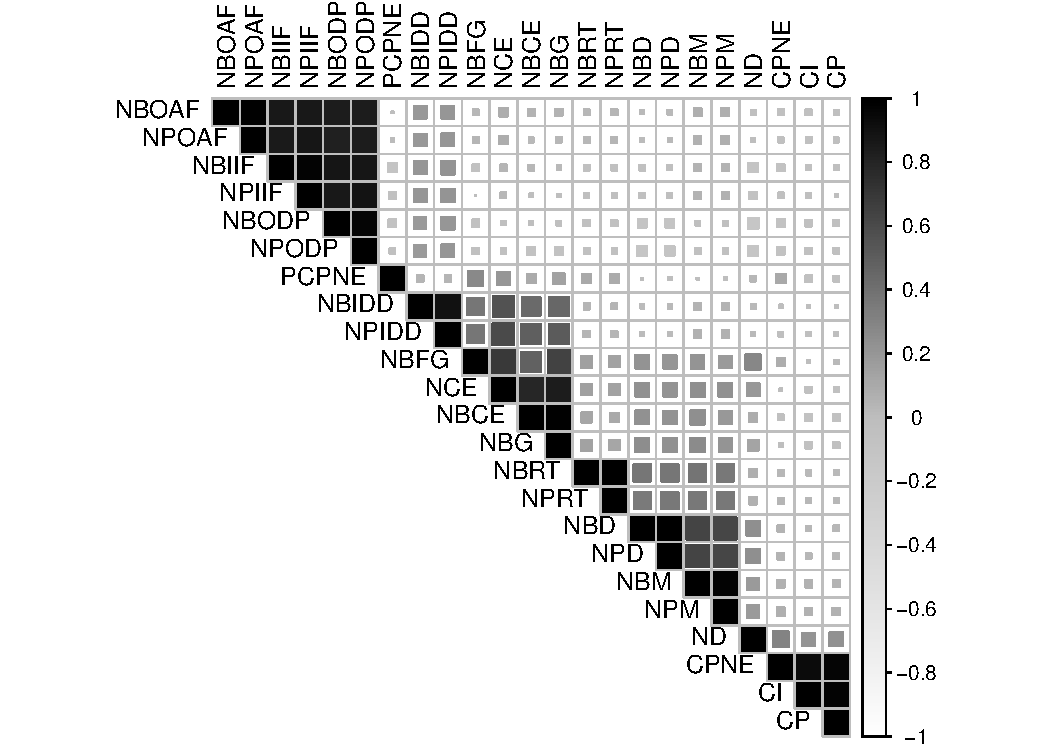
\includegraphics[scale=.75]{../../graficos/latex-graph-matriz-correlacao}
		\caption{Matriz correlograma: correlação entre os pares de variáveis segundo uma escala de cor.}
		\label{fig: matriz-correlograma1}
\end{figure}

Nesta matriz, a ordenação das variáveis foi feita por hierarquia de correlação, ou seja, da esquerda para direita, iniciando pelas correlações mais fortes. Com base na observação nas intensidades das cores, podemos verificar alguns trechos de correlações consideráveis especialmente nas variáveis relacionadas às oportunidades de ampliação da formação e infra-estrutura e instalações físicas.

Na figura \ref{fig: matriz-correlograma-2-bandas} vemos a representação das duas bandas da matriz correlograma. As variáveis assumem ordenamento de acordo com o índice de correlação e são posteriormente agrupadas em \textit{clusters}.

\begin{figure}[H]
		\centering
		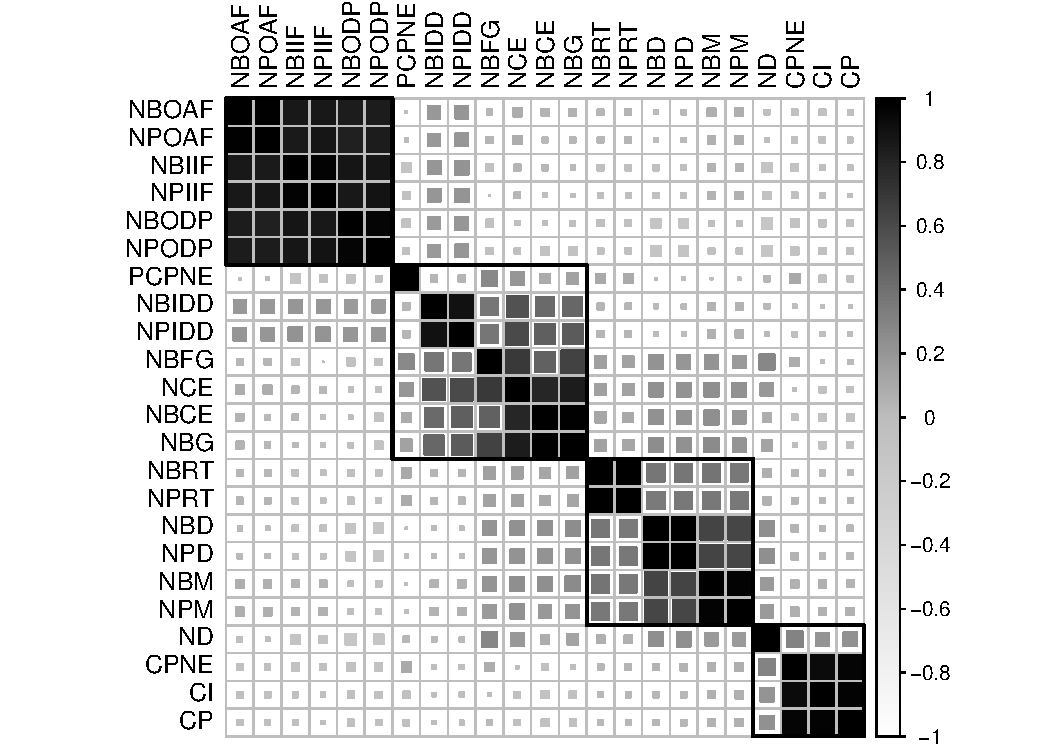
\includegraphics[scale=.75]{../../graficos/latex-graph-matriz-correlacao2.pdf}
		\caption{Matriz correlograma com as duas bandas}
		\label{fig: matriz-correlograma-2-bandas}
\end{figure}

Uma visualização alternativa das correlações pode ser obtida por meio da função \lstinline{shinypairs} do pacote \lstinline{pairsD3}. Este pacote 
permite produzir uma matriz interativa de gráficos de dispersão \cite{pairsD3}. É possível selecionar interativamente, de forma gradual dentre as variáveis preditoras, as que formarão a matriz de correlações. Com base nessa seleção de variáveis, copia-se da tela do \lstinline{shiny}\footnote{Facilitador de visualização interativa de dados. Para maiores informações visitar \url{https://shiny.rstudio.com}} o código que permite replicar a matriz com a função \lstinline{pairs}. 

Na figura \ref{fig: scatter-plot} podemos ver a formação do \textit{scatter-plot} com combinações\footnotemark~ de variáveis obtidas pela interface do \lstinline{pairsD3}.
\footnotetext{É importante observar que, dada a alta quantidade de variáveis contidas na base de dados, não é possível afirmar que a configuração de variáveis mostrada na matriz da figura \ref{fig: scatter-plot} contém combinação de pares com maior correlação. Experimentações foram feitas com variações de pares tendo como referência a matriz correlograma da figura \ref{fig: matriz-correlograma-2-bandas}. Para representação com todas as 23 variáveis preditoras seria necessário espaço suficiente para alocar 529 relações, muito além das dimensões das páginas deste trabalho.}

\begin{figure}[H]
		\centering
		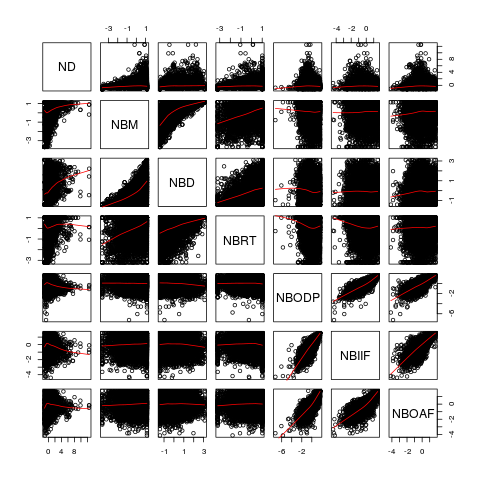
\includegraphics[scale=.80]{../../graficos/latex-graph-pairs.png}
		\caption{Matriz de pares de variáveis}
		\label{fig: scatter-plot}
\end{figure}

Devido ao elevado número de preditoras, esta forma de visualização, apesar de precisa, torna-se prejudicada. Contudo, o diagrama de matriz e a matriz de correlação são duas formas de olhar para a mesma coisa. \cite[p.~98]{larose2015data}

\subsubsection{Aplicação da Análise do Componente Principal}

De acordo com \citeonline[p.~98]{larose2015data} a ACP (Análise do Componente Principal) é a ferramenta mais adequada quando são analisadas variáveis em multicolinearidade. Isto é, tenta-se explicar a estrutura de correlações com base em combinações lineares, também chamadas de componentes. A variabilidade total de todas as variáveis pode ser contabilizada por um conjunto de componentes, uma vez que existe a mesma quantidade de informações nos mesmos em relação ao conjunto original.

Em outras palavras, a análise do componente principal procura reduzir a dimensão de um determinado conjunto de características pela criação de um novo conjunto de propriedades representativas devendo, para tanto, contabilizar a maior variância possível.

\subsubsection{Componentes Principais}

De acordo com \citeonline[p.~95--96]{larose2015data} a ACP é uma técnica de análise que se fundamenta em três corolários:

\begin{enumerate}
\item Assumindo que cada variável preditora possa ser representada em forma de vetor; que o conjunto dessas variáveis tenha sido padronizado e que a quantidade total de variáveis seja $m$, a variabilidade total do grupo de variáveis é igual a soma de cada vetor individual, que é igual à soma dos \textit{eigenvectors\footnotemark}, que é o total de variáveis preditoras. Desta forma, em termos matemáticos temos que:
\footnotetext{Em algebra linear, um \textit{eigenvector} ou vetor característico de uma transformação linear é um vetor não nulo que se altera somente por um fator escalar quando uma transformação linear é aplicada ao mesmo.}

\begin{equation}
\sum_{i=1}^m Var(Y_i) = \sum_{i=1}^m Var(Z_i) = \sum_{i=1}^m \lambda_i = m
\end{equation}

Onde,
\begin{itemize}[label={}]
\item $Y_i$ é o $i$-ésimo componente principal;
\item $Z_i$ é o $i$-ésimo vetor $Z$ (variável preditora pós padronização);
\item $\lambda_i$ é o $i$-ésimo \textit{eigenvector} da variável preditora.
\end{itemize}
\item A proporção de variabilidade total que explica o $i$-ésimo componente principal é a razão entre o $i$-ésimo \textit{eigenvector} pelo total de variáveis, isto é, $\dfrac{\lambda_i}{m}$.
\end{enumerate}

A listagem \ref{lst:loadings_pca} é o resultado da computação e visualização dos componentes principais das 23 preditoras sendo cada célula o peso de um componente:
\pagebreak
\begin{lstlisting}[label={lst:loadings_pca}, captionpos=b, caption={Computação dos carregamentos da Análise do Componente Principal}]
Loadings:
      PC1    PC2    PC3    PC4    PC5   
CI            0.103  0.639  0.722       
CP            0.108  0.642  0.734       
NBFG   0.175  0.624 -0.271  0.234       
NBCE   0.236  0.679 -0.440  0.195       
NBG    0.245  0.732 -0.445  0.223       
NCE    0.285  0.725 -0.430  0.255       
NBODP  0.891 -0.308                     
NPODP  0.891 -0.327  0.112              
NBIIF  0.919 -0.237  0.121              
NPIIF  0.918 -0.237  0.145              
NBOAF  0.918 -0.164  0.140              
NPOAF  0.912 -0.172  0.148              
CPNE          0.152  0.621  0.736       
PCPNE         0.179 -0.124         0.306
NBIDD  0.413  0.379 -0.419  0.331       
NPIDD  0.439  0.399 -0.443  0.334       
ND            0.343  0.232  0.208 -0.197
NBM    0.157  0.653  0.392 -0.343 -0.242
NPM    0.154  0.631  0.410 -0.340 -0.245
NBD           0.670  0.376 -0.373 -0.284
NPD           0.663  0.386 -0.373 -0.284
NBRT          0.497  0.313 -0.334  0.712
NPRT          0.483  0.318 -0.332  0.720

                 PC1   PC2   PC3   PC4   PC5
SS loadings    5.633 4.974 3.207 2.820 1.472
Proportion Var 0.245 0.216 0.139 0.123 0.064
Cumulative Var 0.245 0.461 0.601 0.723 0.787
\end{lstlisting}

Por definição o primeiro componente é o mais representativo de todos, ou seja, é a dimensão que contabiliza a maior variabilidade possível de todas as variáveis preditoras. Em outros termos é a dimensão que maximiza a variância.

Com base na listagem \ref{lst:loadings_pca}, observa-se no primeiro componente (PC1) que as variáveis NBODP, NBIIF e NBOAF tem os maiores pesos. Isso significa que a organização didático pedagógica, infra-estrutura e instalações e oportunidades de ampliação da formação dos estudantes nos cursos são as variáveis mais representativas deste componente. Além disso o primeiro componente contabiliza aproximadamente 1/4 da variância de todo conjunto de componentes.

\subsubsection{Seleção dos Componentes}

A seleção dos componentes pode ser feita com base na seleção de um dentre vários critérios. Um deles é o da proporção da variância explicada que relaciona a área de pesquisa e a proporção de variabilidade que se deseja trabalhar. Em áreas como Ciências Sociais por exemplo, 60\% da variabilidade é considerada satisfatória dada a imprevisibilidade da natureza do comportamento humano \cite[p.~103]{larose2015data}. Sob essa ótica escolheu-se os quatro primeiros componentes, uma vez que os mesmos contabilizam 72,3\% de toda a variabilidade. 

A natureza exploratória da pesquisa fornece relativa liberdade em relação a seleção da quantidade de componentes. Pelo critério \textit{Scree Plot}, a partir do quinto componente é possível verificar uma tendência de estabilização dos pesos, como pode ser observado no gráfico \ref{fig: scree-plot-pca}. Este é o ponto em que se recomenda que seja feita a extração dos componentes.

Sob essa ótica escolheu-se os três primeiros componentes, uma vez que os mesmos contabilizam 60,1\% de toda a variabilidade. Ainda no gráfico \ref{fig: scree-plot-pca}, uma observação pertinente é que pelo critério de \textit{tendência de horizontalização da curva de eigenvalues} sugere-se a possibilidade de selecionar os cinco primeiros componentes. Observa-se que a partir do quinto componente é possível verificar uma tendência de horizontalização da curva de \textit{eigenvalues}. Desta, caso fosse utilizado tal critério seria computada 78,7\% da variabilidade.

\begin{figure}[H]
		\centering
		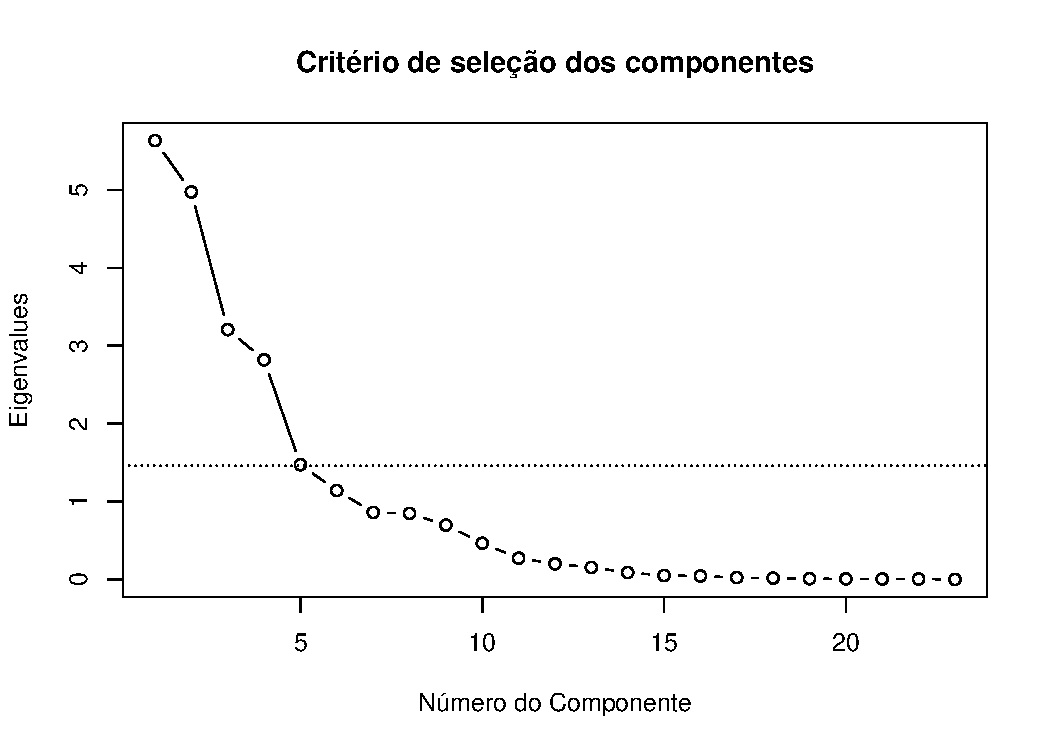
\includegraphics[scale=.80]{../../graficos/latex-graph-scree-plot-pca.pdf}
		\caption{Critério de seleção dos componentes: a partir do 5º componente, observa-se redução no decaimento da variabilidade, o que diminui a importância do componente para uma possível seleção.}
		\label{fig: scree-plot-pca}
\end{figure}

\subsubsection{Características dos Componentes}
A tabela \ref{tbl:caracteristicas-dos-componentes} apresenta com mais clareza os pesos atribuídos aos 4 primeiros componentes pela aplicação da ACP.

% Please add the following required packages to your document preamble:
% \usepackage{booktabs}
\begin{table}[H]
\centering
\begin{tabular}{@{}lllll@{}}
\toprule
\textbf{} & \textbf{PC1} & \textbf{PC2} & \textbf{PC3} & \textbf{PC4} \\ \midrule
CI        & -0.0849      & 0.1032       & 0.6388       & 0.7223       \\
CP        & -0.0748      & 0.1076       & 0.6423       & 0.7344       \\
NBFG      & 0.1748       & 0.6244       & -0.2712      & 0.2344       \\
NBCE      & 0.2362       & 0.6789       & -0.4401      & 0.1951       \\
NBG       & 0.2452       & 0.732        & -0.4448      & 0.2226       \\
NCE       & 0.2849       & 0.7246       & -0.4295      & 0.2552       \\
NBODP     & 0.8914       & -0.3083      & 0.0949       & -0.0112      \\
NPODP     & 0.8906       & -0.327       & 0.1124       & -0.0083      \\
NBIIF     & 0.9189       & -0.2369      & 0.1209       & -0.017       \\
NPIIF     & 0.9185       & -0.2368      & 0.1453       & -0.0077      \\
NBOAF     & 0.9175       & -0.1637      & 0.1402       & -0.033       \\
NPOAF     & 0.9124       & -0.1723      & 0.1478       & -0.03        \\
CPNE      & -0.0899      & 0.1519       & 0.6207       & 0.7365       \\
PCPNE     & -0.0035      & 0.1788       & -0.124       & 0.0935       \\
NBIDD     & 0.4134       & 0.3794       & -0.4194      & 0.3308       \\
NPIDD     & 0.439        & 0.3988       & -0.4431      & 0.3344       \\
ND        & -0.0428      & 0.3428       & 0.2322       & 0.2084       \\
NBM       & 0.1568       & 0.6534       & 0.3918       & -0.3426      \\
NPM       & 0.1542       & 0.6309       & 0.4099       & -0.3402      \\
NBD       & 0.0692       & 0.6702       & 0.3762       & -0.3727      \\
NPD       & 0.0741       & 0.6629       & 0.3857       & -0.3727      \\
NBRT      & 0.0739       & 0.4969       & 0.3134       & -0.334       \\
NPRT      & 0.0727       & 0.4829       & 0.3175       & -0.332       \\ \bottomrule
\end{tabular}
\caption{Características dos Componentes}
\label{tbl:caracteristicas-dos-componentes}
\end{table}

De acordo com \citeonline[p.~107]{larose2015data} o peso dos componentes representa a relação do mesmo com a variável. Para que o peso de um componente tenha significância prática este deve exceder $\pm.50$ em magnitude. Desta forma, a tabela \ref{tbl:caracteristicas-dos-componentes} apresenta a mesma informação, sendo omitidos os pesos menores que 0.5.

% Please add the following required packages to your document preamble:
% \usepackage{booktabs}
\begin{table}[H]
\centering
\begin{tabular}{@{}lllll@{}}
\toprule
\textbf{} & \textbf{PC1} & \textbf{PC2} & \textbf{PC3} & \textbf{PC4} \\ \midrule
CI        &              &              & 0.6388       & 0.7223       \\
CP        &              &              & 0.6423       & 0.7344       \\
NBFG      &              & 0.6244       &              &              \\
NBCE      &              & 0.6789       &              &              \\
NBG       &              & 0.732        &              &              \\
NCE       &              & 0.7246       &              &              \\
NBODP     & 0.8914       &              &              &              \\
NPODP     & 0.8906       &              &              &              \\
NBIIF     & 0.9189       &              &              &              \\
NPIIF     & 0.9185       &              &              &              \\
NBOAF     & 0.9175       &              &              &              \\
NPOAF     & 0.9124       &              &              &              \\
CPNE      &              &              & 0.6207       & 0.7365       \\
PCPNE     &              &              &              &              \\
NBIDD     &              &              &              &              \\
NPIDD     &              &              &              &              \\
ND        &              &              &              &              \\
NBM       &              & 0.6534       &              &              \\
NPM       &              & 0.6309       &              &              \\
NBD       &              & 0.6702       &              &              \\
NPD       &              & 0.6629       &              &              \\
NBRT      &              &              &              &              \\
NPRT      &              &              &              &              \\ \bottomrule
\end{tabular}
\caption{Componentes com magnitudes $\pm.50$}
\label{my-label}
\end{table}

Determinados os pesos, é possível agora classificar os componentes principais de acordo com sua estrutura e pesos nas variáveis:

\begin{enumerate}
\item O primeiro componente (PC1) apresenta pesos significativos nas variáveis  \textit{Organização Didático-pedagógica}, \textit{Infra-estrutura e Instalações} e \textit{Oportunidades de Ampliação da Formação}. Com base nisto é possível concluir que esse componente apresenta um perfil do que o curso é capaz de entregar ao aluno, que é refletida nas notas que o mesmo atribui no momento da avaliação.
\item Em PC2 observamos uma concentração dos pesos nas variáveis associadas a duas dimensões: alunos e professores. No que se refere aos alunos, pesam mais as notas avaliadas de acordo com o desempenho dos mesmos nas provas nas áreas de \textit{Formação Geral} e \textit{Conhecimentos Específicos}. Já em relação aos professores tem destaque as variáveis \textit{Quantidade de Mestres} e \textit{Quantidade de Doutores} nos cursos.
\item Em PC3 têm destaque as variáveis \textit{Concluíntes Inscritos} e \textit{Percentual de Concluíntes Participantes com nota no Enem}. Isso indica que este componente tem um perfil mais voltado a determinar a situação dos alunos no censo bem como a contabilização da participação dos mesmos.
\item PC4 apresenta perfil de composição similar à PC3. Os pesos, por sua vez, apresentam magnitudes levemente superiores. Isso se deve ao fato de esse componente ter tido uma proporção de variância individual menor em relação a PC3 (13,9\% contra 21,6\%) como pode ser observado na listagem \ref{lst:loadings_pca}. Desta forma, apesar de este componente ter apresentado pesos relativamente maiores, sua variância total menor faz com que seja posicionado em 4º na ordem dos componentes.
\end{enumerate}

%Enviado para a sessão Resultados, após comentário no Schoology em 10/7 às 9:39 am.
%Por meio da aplicação da análise do componente principal foi possível identificar características relevantes sobre as variáveis preditoras do CPC. A referida análise também possibilitou o agrupamento destas variáveis em componentes principais. Verificou-se que o primeiro (principal) componente apresenta afinidade com o que o curso e a instituição de ensino dipõem em termos de profissionais (Organização Didático-pedagógica), estrutura (Infra-estrutura e Instalações) e perspectiva do futuro, do ponto de vista do aluno (Oportunidades de Ampliação da Formação). A pontuação nestas variáveis tem origem em avaliação subjetiva do aluno participante do censo. A classificação destas variáveis como constantes no primeiro componente permite-nos afirmar que um maior desempenho nestes quesitos implicará em maior resposta na variável dependente (CPC Contínuo).
